% Created by tikzDevice version 0.12.3.1 on 2022-09-19 22:27:53
% !TEX encoding = UTF-8 Unicode
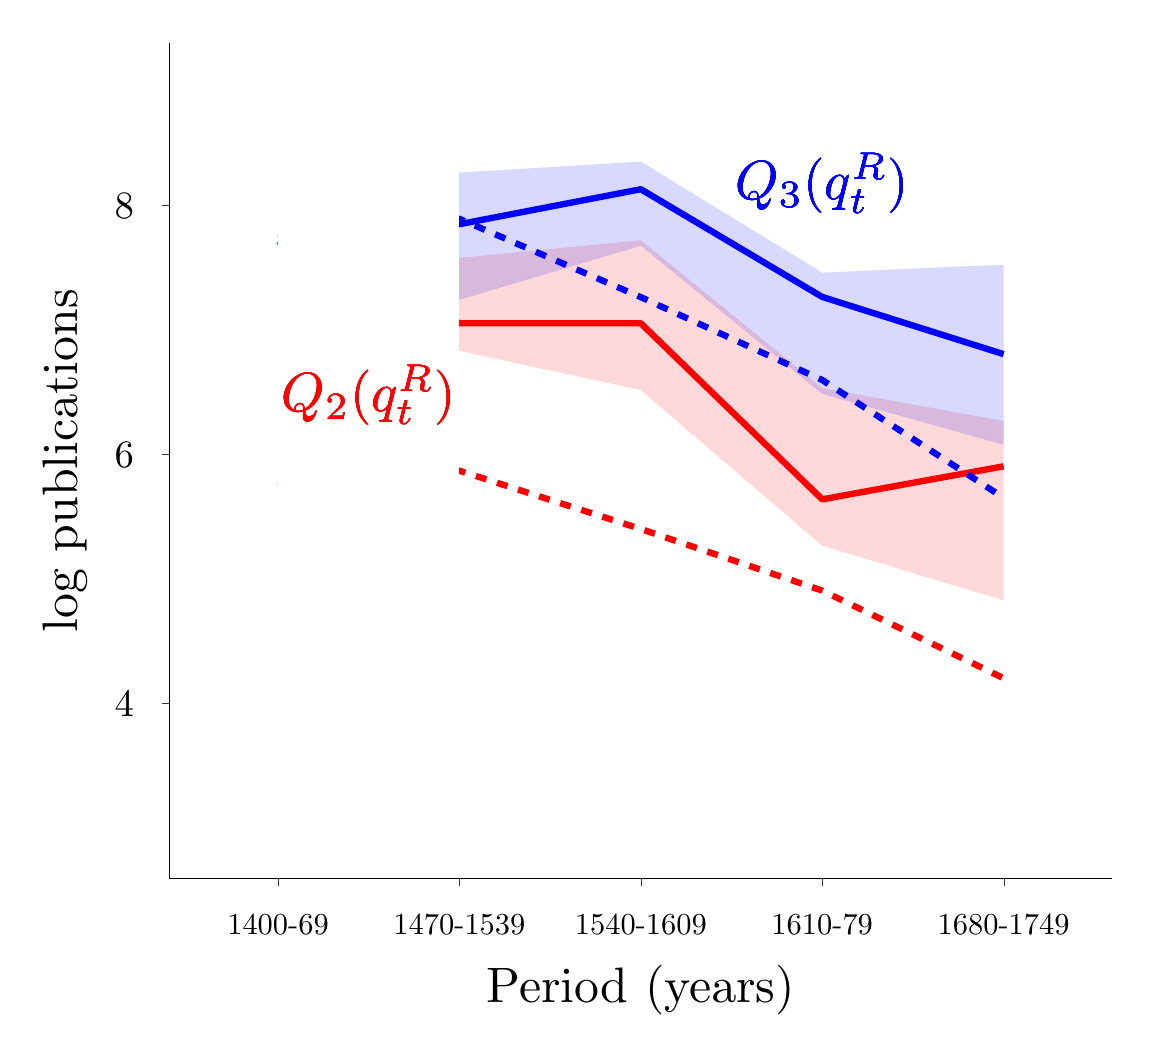
\begin{tikzpicture}[x=1pt,y=1pt]
\definecolor{fillColor}{RGB}{255,255,255}
\path[use as bounding box,fill=fillColor,fill opacity=0.00] (0,0) rectangle (397.48,361.35);
\begin{scope}
\path[clip] (  0.00,  0.00) rectangle (397.48,361.35);
\definecolor{drawColor}{RGB}{255,255,255}
\definecolor{fillColor}{RGB}{255,255,255}

\path[draw=drawColor,line width= 0.1pt,line join=round,line cap=round,fill=fillColor] (  0.00,  0.00) rectangle (397.48,361.35);
\end{scope}
\begin{scope}
\path[clip] ( 51.14, 53.86) rectangle (391.98,355.85);
\definecolor{fillColor}{RGB}{255,255,255}

\path[fill=fillColor] ( 51.14, 53.86) rectangle (391.98,355.85);
\definecolor{fillColor}{RGB}{255,0,0}

\path[fill=fillColor,fill opacity=0.15] ( 90.47,292.14) --
	(156.02,278.15) --
	(221.56,284.53) --
	(287.11,231.13) --
	(352.66,219.22) --
	(352.66,154.37) --
	(287.11,174.15) --
	(221.56,230.40) --
	(156.02,244.55) --
	( 90.47,254.76) --
	cycle;

\path[] ( 90.47,292.14) --
	(156.02,278.15) --
	(221.56,284.53) --
	(287.11,231.13) --
	(352.66,219.22);

\path[] (352.66,154.37) --
	(287.11,174.15) --
	(221.56,230.40) --
	(156.02,244.55) --
	( 90.47,254.76);
\definecolor{drawColor}{RGB}{255,0,0}

\path[draw=drawColor,line width= 2.3pt,line join=round] ( 90.47,284.23) --
	(156.02,254.56) --
	(221.56,254.52) --
	(287.11,190.91) --
	(352.66,202.85);

\path[draw=drawColor,line width= 2.3pt,dash pattern=on 4pt off 4pt ,line join=round] ( 90.47,195.87) --
	(156.02,201.25) --
	(221.56,180.20) --
	(287.11,157.93) --
	(352.66,126.27);
\definecolor{fillColor}{RGB}{0,0,255}

\path[fill=fillColor,fill opacity=0.15] ( 90.47,325.49) --
	(156.02,308.99) --
	(221.56,312.95) --
	(287.11,272.84) --
	(352.66,275.70) --
	(352.66,210.60) --
	(287.11,228.99) --
	(221.56,282.55) --
	(156.02,262.97) --
	( 90.47,278.47) --
	cycle;

\path[] ( 90.47,325.49) --
	(156.02,308.99) --
	(221.56,312.95) --
	(287.11,272.84) --
	(352.66,275.70);

\path[] (352.66,210.60) --
	(287.11,228.99) --
	(221.56,282.55) --
	(156.02,262.97) --
	( 90.47,278.47);
\definecolor{drawColor}{RGB}{0,0,255}

\path[draw=drawColor,line width= 2.3pt,line join=round] ( 90.47,291.49) --
	(156.02,290.33) --
	(221.56,302.97) --
	(287.11,264.05) --
	(352.66,243.37);

\path[draw=drawColor,line width= 2.3pt,dash pattern=on 4pt off 4pt ,line join=round] ( 90.47,285.04) --
	(156.02,292.27) --
	(221.56,263.97) --
	(287.11,234.03) --
	(352.66,191.46);
\definecolor{fillColor}{RGB}{255,255,255}

\path[fill=fillColor] ( 90.47, 53.86) rectangle (156.02,355.85);

\path[fill=fillColor] ( 90.47, 53.86) rectangle (156.02,355.85);

\path[fill=fillColor] ( 90.47, 53.86) rectangle (156.02,355.85);

\path[fill=fillColor] ( 90.47, 53.86) rectangle (156.02,355.85);

\path[fill=fillColor] ( 90.47, 53.86) rectangle (156.02,355.85);

\node[text=drawColor,anchor=base,inner sep=0pt, outer sep=0pt, scale=  1.99] at (287.11,299.26) {$Q_3(q_t^R)$};

\node[text=drawColor,anchor=base,inner sep=0pt, outer sep=0pt, scale=  1.99] at (287.11,299.26) {$Q_3(q_t^R)$};

\node[text=drawColor,anchor=base,inner sep=0pt, outer sep=0pt, scale=  1.99] at (287.11,299.26) {$Q_3(q_t^R)$};

\node[text=drawColor,anchor=base,inner sep=0pt, outer sep=0pt, scale=  1.99] at (287.11,299.26) {$Q_3(q_t^R)$};

\node[text=drawColor,anchor=base,inner sep=0pt, outer sep=0pt, scale=  1.99] at (287.11,299.26) {$Q_3(q_t^R)$};
\definecolor{drawColor}{RGB}{255,0,0}

\node[text=drawColor,anchor=base,inner sep=0pt, outer sep=0pt, scale=  1.99] at (123.25,222.75) {$Q_2(q_t^R)$};

\node[text=drawColor,anchor=base,inner sep=0pt, outer sep=0pt, scale=  1.99] at (123.25,222.75) {$Q_2(q_t^R)$};

\node[text=drawColor,anchor=base,inner sep=0pt, outer sep=0pt, scale=  1.99] at (123.25,222.75) {$Q_2(q_t^R)$};

\node[text=drawColor,anchor=base,inner sep=0pt, outer sep=0pt, scale=  1.99] at (123.25,222.75) {$Q_2(q_t^R)$};

\node[text=drawColor,anchor=base,inner sep=0pt, outer sep=0pt, scale=  1.99] at (123.25,222.75) {$Q_2(q_t^R)$};
\end{scope}
\begin{scope}
\path[clip] (  0.00,  0.00) rectangle (397.48,361.35);
\definecolor{drawColor}{RGB}{0,0,0}

\path[draw=drawColor,line width= 0.1pt,line join=round] ( 51.14, 53.86) --
	( 51.14,355.85);
\end{scope}
\begin{scope}
\path[clip] (  0.00,  0.00) rectangle (397.48,361.35);
\definecolor{drawColor}{RGB}{0,0,0}

\node[text=drawColor,anchor=base east,inner sep=0pt, outer sep=0pt, scale=  1.40] at ( 38.39,112.27) {4};

\node[text=drawColor,anchor=base east,inner sep=0pt, outer sep=0pt, scale=  1.40] at ( 38.39,202.28) {6};

\node[text=drawColor,anchor=base east,inner sep=0pt, outer sep=0pt, scale=  1.40] at ( 38.39,292.30) {8};
\end{scope}
\begin{scope}
\path[clip] (  0.00,  0.00) rectangle (397.48,361.35);
\definecolor{drawColor}{gray}{0.20}

\path[draw=drawColor,line width= 0.1pt,line join=round] ( 48.39,117.09) --
	( 51.14,117.09);

\path[draw=drawColor,line width= 0.1pt,line join=round] ( 48.39,207.11) --
	( 51.14,207.11);

\path[draw=drawColor,line width= 0.1pt,line join=round] ( 48.39,297.12) --
	( 51.14,297.12);
\end{scope}
\begin{scope}
\path[clip] (  0.00,  0.00) rectangle (397.48,361.35);
\definecolor{drawColor}{RGB}{0,0,0}

\path[draw=drawColor,line width= 0.1pt,line join=round] ( 51.14, 53.86) --
	(391.98, 53.86);
\end{scope}
\begin{scope}
\path[clip] (  0.00,  0.00) rectangle (397.48,361.35);
\definecolor{drawColor}{gray}{0.20}

\path[draw=drawColor,line width= 0.1pt,line join=round] ( 90.47, 51.11) --
	( 90.47, 53.86);

\path[draw=drawColor,line width= 0.1pt,line join=round] (156.02, 51.11) --
	(156.02, 53.86);

\path[draw=drawColor,line width= 0.1pt,line join=round] (221.56, 51.11) --
	(221.56, 53.86);

\path[draw=drawColor,line width= 0.1pt,line join=round] (287.11, 51.11) --
	(287.11, 53.86);

\path[draw=drawColor,line width= 0.1pt,line join=round] (352.66, 51.11) --
	(352.66, 53.86);
\end{scope}
\begin{scope}
\path[clip] (  0.00,  0.00) rectangle (397.48,361.35);
\definecolor{drawColor}{RGB}{0,0,0}

\node[text=drawColor,anchor=base,inner sep=0pt, outer sep=0pt, scale=  1.10] at ( 90.47, 33.53) {1400-69};

\node[text=drawColor,anchor=base,inner sep=0pt, outer sep=0pt, scale=  1.10] at (156.02, 33.53) {1470-1539};

\node[text=drawColor,anchor=base,inner sep=0pt, outer sep=0pt, scale=  1.10] at (221.56, 33.53) {1540-1609};

\node[text=drawColor,anchor=base,inner sep=0pt, outer sep=0pt, scale=  1.10] at (287.11, 33.53) {1610-79};

\node[text=drawColor,anchor=base,inner sep=0pt, outer sep=0pt, scale=  1.10] at (352.66, 33.53) {1680-1749};
\end{scope}
\begin{scope}
\path[clip] (  0.00,  0.00) rectangle (397.48,361.35);
\definecolor{drawColor}{RGB}{0,0,0}

\node[text=drawColor,anchor=base,inner sep=0pt, outer sep=0pt, scale=  1.80] at (221.56,  9.00) {Period (years)};
\end{scope}
\begin{scope}
\path[clip] (  0.00,  0.00) rectangle (397.48,361.35);
\definecolor{drawColor}{RGB}{0,0,0}

\node[text=drawColor,rotate= 90.00,anchor=base,inner sep=0pt, outer sep=0pt, scale=  1.80] at ( 17.90,204.86) {log publications};
\end{scope}
\end{tikzpicture}
